\begin{frame}
    \fta{Mehrphasensysteme - Mitsystem, Gegensystem und Nullsystem}

    \s{
        Im Kapitel Drehstrom wurde erläutert, wie sich die Spannungen, die Ströme und die Leistungen in verschiedenen dreiphäsigen Systemen zusammensetzen.
        In dem besonderen Fall von symmetrischen Verbrauchern konnte gezeigt werden, dass relativ einfach eine Netzberechnung druchgeführt werden kann.
        Vor allem die vereinfachte Darstellung durch die einphasigen Ersatzschaltbilder hilft bei der Berechnung.
        Durch unsymmetrische Verbraucher können diese Vereinfachungen nicht angenommen werden und führen dazu, dass umfassendere Netzberechnungen auch schon bei kleinen Netzen unübersichtlich und aufwändig werden.
        Unsymmetrien treten z.B. durch Netzfehler wie ein einpoliger Kurzschluss, durch Schalthandlungen, oder unsymmetrische Belastung der einzelnen Phasen auf.
        Die Zusammenhänge von auslösenden Ereignissen und den Ergebnissen sind allein anhand von Zahlenwerten schwer nachvollziehbar.
        Um auch umfassende und unsymmetrische Netze berechnen zu können, kann mit einer Transformation des bekannten Systems in drei neue Systeme abhilfe geschaffen werden.
        Dafür werden die drei folgenden Systeme näher betrachtet: 
    }

    \begin{Lernziele}{Mehrphasensysteme}
        Die Studierenden
        \begin{itemize}
            \item verstehen die Funktionen von Mit-, Gegen- und Nullsystem. 
            \item können die Drehstromleistung der verschiedenen Systeme berechnen.
            \item können Ersatzschaltbilder für symmetrische Quellen, Lasten und Leitungen erstellen. 
        \end{itemize}
    \end{Lernziele}
   
\end{frame}




\begin{frame}
    \ftx{Methode der symmetrischen Komponenten}
    \b{
        Um eine solche Transformation sinnvoll einzusetzen, sollten gewisse Forderungen erfüllt werden:
        
    \begin{itemize}
        \item [1.]Die Berechnung im transformierten System müssen einfacher sein als im Originalsystem
        \item [2.]Die Symmetrien der realen Netze und Betriebsmittel müssen vorteilhaft genutzt werden
        \item [3.]Es müssen sowohl Ströme als auch Spannungen mit den gleichen Transformationsvorschriften behandelt werden
        \item [4.]Die Leistungen sollen in beiden Systemen identisch sein, falls das nicht möglich ist sollen die Leistungen über einen konstanten Faktor umzurechnen sein
    \end{itemize}
    }
\end{frame}





\begin{frame}
    \ftb{Mit-, Gegen- und Nullsystem}

    \s{
        Grundlegend ist das Ziel der Transformation, ein unsymmetrisches System von n Zeigern in n Systeme mit symmetrischer Zeigeranordnung zu überführen.
        Für ein Drehstromsystem bedeutet das, dass drei Systeme geschaffen werden sollen.
        Jeder Leiter, also $L_1$, $L_2$ und $L_3$ soll ersetzt werden durch ein System was eine symmetrische Zeigeranordnung hat.
        Grundlage der Transformationsvorschrift ist der bereits bekannte Drehoperator $\underline{a}$ und $\underline{a}^2$ (vgl. Gleichung \ref{Drehoperator}).
        Für den Strom in den jeweiligen Leitern lassen sich so die Symmetriebedingungen aufstellen (Hier ist anzumerken, dass alles was für den Strom gilt an Zusammenhängen auch für die Spannung gilt!):
        
        \begin{eqa}
            \underline{I}_{\mathrm{L1}}&=\underline{I}_{0}+\underline{I}_{1}+\underline{I}_{2} \nonumber \\
            \underline{I}_{\mathrm{L2}}&=\underline{I}_{0}+\underline{a}^2\cdot \underline{I}_{1}+\underline{a}\cdot\underline{I}_{2} \label{ZerlegungL2} \\
            \underline{I}_{\mathrm{L3}}&=\underline{I}_{0}+\underline{a}\cdot\underline{I}_{1}+\underline{a}^2\cdot\underline{I}_{2} \nonumber
        \end{eqa}

        Die Indizes den rechten Seiten der Gleichungen stehen für die drei Systeme: Mitsystem (1), Gegensystem (2) und Nullsystem (0).
        Schaut man sich die Werte des Mitsystems an, dann ergeben sich durch die Drehoperatoren rechtsdrehende Phasenströme.
        Bei dem Gegensystem sind die transformierten Phasenströme linksdrehend angeordnet und bei dem Nullsystem sind alle Komponenten gleichgerichtet.
        Grundsätzlich tritt das Nullsystem nur dann auf, wenn die Summe aller Ströme des Ausgangssystems ungleich Null sind.
    }

    \b{
        \begin{itemize}
            \item Ziel der Transformation ist, ein unsymmetrisches System von n Zeigern in n Systeme mit symmetrischer Zeigeranordnung zu überführen
            \item Im Drehstrom bekommt jeder Leiter ($L_1, L_2, L_3$) ein System mit symmetrischer Zeigeranordnung
            \item Mit Hilfe des Drehoperators lassen sich Symmetriebedingungen für jeden Leiter aufstellen, die sogenannten Zerlegungsgleichungen:
        \end{itemize}
        \begin{eqa}
            \underline{I}_{\mathrm{L1}}&=\underline{I}_{0}+\underline{I}_{1}+\underline{I}_{2} \\
            \underline{I}_{\mathrm{L2}}&=\underline{I}_{0}+\underline{a}^2\cdot \underline{I}_{1}+\underline{a}\cdot\underline{I}_{2} \\
            \underline{I}_{\mathrm{L3}}&=\underline{I}_{0}+\underline{a}\cdot\underline{I}_{1}+\underline{a}^2\cdot\underline{I}_{2} 
        \end{eqa}
        Hier ist anzumerken, dass alles was für den Strom gilt an Zusammenhängen auch für die Spannung gilt!
    }
\end{frame}




\begin{frame}
    \ftx{Grundlagen - Zerlegungsgleichungen}
    \s{
    Im nächsten Schritt werden die sogenannten Zerlegungsgleichungen (Gleichungen \ref{ZerlegungL2}) so umgestellt, dass das Verhältnisse vom Strom des Mit- Gegen- Nullsystemes zu den Leiterströmen des Ursprungssytem aufzeigt wird.

    Für den Strom im Nullsystem gilt durch Addition:

    \begin{eqa}
        \underline{I}_{\mathrm{L1}}+\underline{I}_{\mathrm{L2}}+\underline{I}_{\mathrm{L3}}&=3\cdot\underline{I}_0+\underline{I}_1\cdot(1+\underline{a}^2+\underline{a})+\underline{I}_2\cdot(1+\underline{a}+\underline{a}^2) \notag \\
        &=3\cdot\underline{I}_0 \\
        \Leftrightarrow      \underline{I}_0&=\frac{1}{3}\cdot(\underline{I}_{\mathrm{L1}}+\underline{I}_{\mathrm{L2}}+\underline{I}_{\mathrm{L3}})
    \end{eqa}

    
    Für die Ermittlung des Stroms des Mitsystems werden zuerst die Gleichungen so multipliziert, dass die Vorfaktoren vor dem Mitstrom 1 ergeben.
    Danach werden die Zerlegungsgleichungen wieder addiert.

    $\underline{a}^3=1$  ;  $\underline{a}^4=\underline{a}$  ;  $\underline{a}^5=\underline{a}^2$  ;  ...

    \begin{eqa}
        \underline{I}_{\mathrm{L1}}&=\underline{I}_{0}+\underline{I}_{1}+\underline{I}_{2} \\
        \underline{a}\cdot\underline{I}_{\mathrm{L2}}&=\underline{a}\cdot\underline{I}_{0}+\underline{a}^3\cdot \underline{I}_{1}+\underline{a}^2\cdot\underline{I}_{2} \\
        \underline{a}^2\cdot\underline{I}_{\mathrm{L3}}&=\underline{a}^2\cdot\underline{I}_{0}+\underline{a}^3\cdot\underline{I}_{1}+\underline{a}\cdot\underline{I}_{2}   
    \end{eqa}

    \begin{eqa}
        \underline{I}_{\mathrm{L1}}+\underline{a}\cdot\underline{I}_{\mathrm{L2}}+\underline{a}^2\cdot\underline{I}_{\mathrm{L3}}&=\underline{I}_{0}\cdot(1+\underline{a}+\underline{a}^2)+3\cdot\underline{I}_{1}+\underline{I}_{2}\cdot(1+\underline{a}^2+\underline{a})  \\
        &=3\cdot\underline{I}_{1}  \notag\\
        \Leftrightarrow \underline{I}_{1}&=\frac{1}{3}\cdot(\underline{I}_{\mathrm{L1}}+\underline{a}\cdot\underline{I}_{\mathrm{L2}}+\underline{a}^2\cdot\underline{I}_{\mathrm{L3}}) \notag
    \end{eqa}

    Zum Schluss wird noch der Strom für das Gegensystem berechnet.
    Dabei wird das gleiche Prinzip angewendet, wie beim Mitsystem: Erst wird der Vorfaktor angepasst, dann alle Zerlegungsgleichungen addiert:

    \begin{eqa}
        \underline{I}_{\mathrm{\mathrm{L1}}}&=\underline{I}_{0}+\underline{I}_{1}+\underline{I}_{2} \\
        \underline{a}^2\cdot\underline{I}_{\mathrm{\mathrm{L2}}}&=\underline{a}^2\cdot\underline{I}_{0}+\underline{a}^4\cdot \underline{I}_{1}+\underline{a}^3\cdot\underline{I}_{2} \\
        \underline{a}\cdot\underline{I}_{\mathrm{\mathrm{L3}}}&=\underline{a}\cdot\underline{I}_{0}+\underline{a}^2\cdot\underline{I}_{1}+\underline{a}^3\cdot\underline{I}_{2}   
    \end{eqa}

    \begin{eqa}
        \underline{I}_{\mathrm{L1}}+\underline{a}^2\cdot\underline{I}_{\mathrm{L2}}+\underline{a}\cdot\underline{I}_{\mathrm{L3}}&=(1+\underline{a}^2+\underline{a})\underline{I}_{0}+(1+\underline{a}+\underline{a}^2)\cdot\underline{I}_{1}+3\cdot\underline{I}_{2}  \\
        &=3\cdot\underline{I}_{2} \notag\\
        \Leftrightarrow \underline{I}_{2}&=\frac{1}{3}\cdot(\underline{I}_{\mathrm{L1}}+\underline{a}^2\cdot\underline{I}_{\mathrm{L2}}+\underline{a}\cdot\underline{I}_{\mathrm{L3}}) \notag
    \end{eqa}

    So ergeben sich für die Ströme aller System folgende Gleichungen:
    
    \begin{eqa}
        \underline{I}_0&=\frac{1}{3}\cdot(\underline{I}_{\mathrm{L1}}+\underline{I}_{\mathrm{L2}}+\underline{I}_{\mathrm{L3}}) \\
        \underline{I}_{1}&=\frac{1}{3}\cdot(\underline{I}_{\mathrm{L1}}+\rlap{\underline{a}}\phantom{a^2}\cdot\underline{I}_{\mathrm{L2}}+\underline{a}^2\cdot\underline{I}_{\mathrm{L3}}) \\
        \underline{I}_{2}&=\frac{1}{3}\cdot(\underline{I}_{\mathrm{L1}}+\underline{a}^2\cdot\underline{I}_{\mathrm{L2}}+\rlap{\underline{a}}\phantom{a^2}\cdot\underline{I}_{\mathrm{L3}})
    \end{eqa}

    Schaut man sich diese drei Gleichungen genau an, sieht man, dass der Leiter L1 in keiner der drei Gleichungen einen Drehoperator als Vorfaktor hat.
    Deshalb soll der L1 Leiter als Bezugsleiter gewählt werden.
    Das bedeutet, dass das der Leiter ist, durch den eine Unsymmetrie im Originalsystem auftritt (z.B. durch einen einpoligen Erdkurzschluss).
    Die vorhanden Restsymmetrien im Originalsystem können dann einfacher über die anderen Leiter betrachtet werden
    Es kann natürlich jeder Leiter als Bezugsleiter genommen werden, da grundsätzlich jeder Leiter einem Index (L1, L2, L3) frei zugeordnet werden kann.
    So kann jedoch die anfänglich festgelegte Vorderung erfüllt werden: Die Symmetrien der realen Netze und Betriebsmittel müssen vorteilhaft genutzt werden!
    }

    \b{
        \begin{itemize}
            \item Die Zerlegungsgleichungen sollen im nächsten Schritt gleichgesetzt werden und zum Strom des jeweiligen Systems umgesetellt werden
            \item Für das Nullsystem ergibt dies folgende Gleichung:
        \end{itemize}
        \begin{eqa}
            \underline{I}_{\mathrm{L1}}+\underline{I}_{\mathrm{L2}}+\underline{I}_{\mathrm{L3}}&=3\cdot\underline{I}_0+\underline{I}_1\cdot(1+\underline{a}^2+\underline{a})+\underline{I}_2\cdot(1+\underline{a}+\underline{a}^2) \notag \\
            &=3\cdot\underline{I}_0 \\
            \Leftrightarrow      \underline{I}_0&=\frac{1}{3}\cdot(\underline{I}_{\mathrm{L1}}+\underline{I}_{\mathrm{L2}}+\underline{I}_{\mathrm{L3}})
        \end{eqa}
    }

\end{frame}

    \begin{frame}
        \ftx{Grundlagen - Zerlegungsgleichungen}

\b{
    \begin{itemize}
                \item Um die addierten Ströme für den Strom des Mitsystems umzustellen, muss ein Zwischenschritt gemacht werden
                \item Es soll zuerst der Drehoperator aus dem Vorfaktor gerechnet werden, indem mit dem passend Drehoperatoren multipliziert wird:
    \end{itemize}            
    \begin{eqa}
        \underline{I}_{\mathrm{L1}}&=\underline{I}_{0}+\underline{I}_{1}+\underline{I}_{2} \\
        \underline{a}\cdot\underline{I}_{\mathrm{L2}}&=\underline{a}\cdot\underline{I}_{0}+\underline{a}^3\cdot \underline{I}_{1}+\underline{a}^2\cdot\underline{I}_{2} \\
        \underline{a}^2\cdot\underline{I}_{\mathrm{L3}}&=\underline{a}^2\cdot\underline{I}_{0}+\underline{a}^3\cdot\underline{I}_{1}+\underline{a}\cdot\underline{I}_{2}   
    \end{eqa}
    \begin{eqa}
        \underline{I}_{\mathrm{L1}}+\underline{a}\cdot\underline{I}_{\mathrm{L2}}+\underline{a}^2\cdot\underline{I}_{\mathrm{L3}}&=\underline{I}_{0}\cdot(1+\underline{a}+\underline{a}^2)+3\cdot\underline{I}_{1}+\underline{I}_{2}\cdot(1+\underline{a}^2+\underline{a})  \\
        &=3\cdot\underline{I}_{1}  \notag\\
        \Leftrightarrow \underline{I}_{1}&=\frac{1}{3}\cdot(\underline{I}_{L1}+\underline{a}\cdot\underline{I}_{L2}+\underline{a}^2\cdot\underline{I}_{L3}) \notag
    \end{eqa} 
    }
    \end{frame}

\begin{frame}
    \ftx{Grundlagen - Zerlegungsgleichungen}
    \b{
        \begin{itemize}
            \item Der Strom für das Gegensystem errechnet sich äquivalent zum Mitsystem:
        \end{itemize}
        \begin{eqa}
            \underline{I}_{\mathrm{\mathrm{L1}}}&=\underline{I}_{0}+\underline{I}_{1}+\underline{I}_{2} \\
            \underline{a}^2\cdot\underline{I}_{\mathrm{\mathrm{L2}}}&=\underline{a}^2\cdot\underline{I}_{0}+\underline{a}^4\cdot \underline{I}_{1}+\underline{a}^3\cdot\underline{I}_{2} \\
            \underline{a}\cdot\underline{I}_{\mathrm{\mathrm{L3}}}&=\underline{a}\cdot\underline{I}_{0}+\underline{a}^2\cdot\underline{I}_{1}+\underline{a}^3\cdot\underline{I}_{2}   
        \end{eqa}
        \begin{eqa}
            \underline{I}_{\mathrm{L1}}+\underline{a}^2\cdot\underline{I}_{\mathrm{L2}}+\underline{a}\cdot\underline{I}_{\mathrm{L3}}&=(1+\underline{a}^2+\underline{a})\underline{I}_{0}+(1+\underline{a}+\underline{a}^2)\cdot\underline{I}_{1}+3\cdot\underline{I}_{2}  \\
            &=3\cdot\underline{I}_{2} \notag\\
            \Leftrightarrow \underline{I}_{2}&=\frac{1}{3}\cdot(\underline{I}_{\mathrm{L1}}+\underline{a}^2\cdot\underline{I}_{\mathrm{L2}}+\underline{a}\cdot\underline{I}_{\mathrm{L3}}) \notag
        \end{eqa}
    }
\end{frame}
    
\begin{frame}
    \ftx{Zeigerdiagramm eines unsymmetrischen Stroms im Dreiphasensystem und die Transformationen}
    
\s{
    Beispielhaft kann ein unsymmetrischer Strom im Dreiphasensytem und die Transformation folgendermaßen aussehen:
}

    \fu{\resizebox{0.6\textwidth}{!}{%
        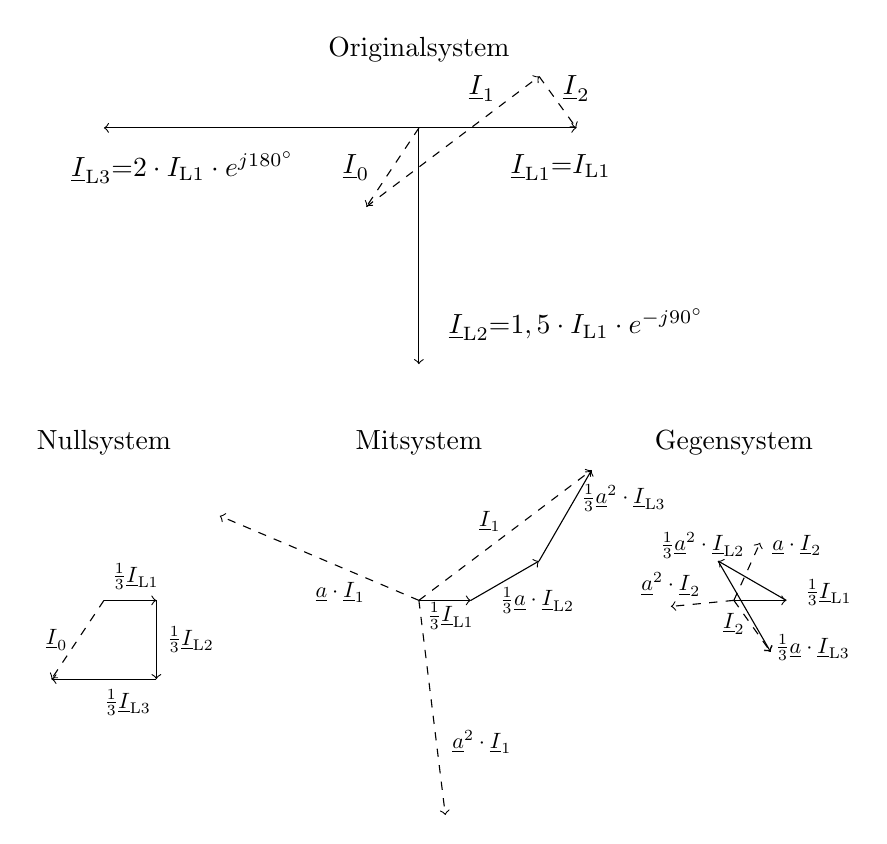
\begin{tikzpicture}
    \draw [->] (0, 0) -- (2, 0);
    \draw [->] (0, 0) -- (-4, 0);
    \draw [->] (0, 0) -- (0, -3);
    \draw [->] [dashed] (0, 0) -- (-0.666, -1);
    \draw [->] [dashed] (-0.666, -1) -- (1.527, 0.654);
    \draw [->] [dashed] (1.527, 0.654) -- (2, 0);

    \draw (1.8, -0.5) node {$\underline{I}_{\mathrm{L1}}{=}I_\mathrm{L1}$};
    \draw (-3, -0.5) node {$\underline{I}_{\mathrm{L3}}{=}2\cdot I_\mathrm{L1}\cdot e^{j180^{\circ}}$};
    \draw (2, -2.5) node {$\underline{I}_{\mathrm{L2}}{=}1,5\cdot I_\mathrm{L1}\cdot e^{-j90^{\circ}}$};
    \draw (0.8, 0.5) node {$\underline{I}_{\mathrm{1}}$};
    \draw (2, 0.5) node {$\underline{I}_{\mathrm{2}}$};
    \draw (-0.8, -0.5) node {$\underline{I}_{\mathrm{0}}$};

    \draw [->] [dashed] (0, -6) -- (2.193, -4.346);
    \draw [->] [dashed] (0, -6) -- (-2.529, -4.927);
    \draw [->] [dashed] (0, -6) -- (0.336, -8.726);
    \draw [->] (0, -6) -- (0.66, -6);
    \draw [->] (0.66, -6) -- (1.526, -5.5);
    \draw [->] (1.526, -5.5) -- (2.193, -4.346);

    \draw (0.9, -5) node [scale=0.8] {$\underline{I}_{\mathrm{1}}$};
    \draw (-1, -5.9) node [scale=0.8] {$\underline{a}\cdot\underline{I}_{\mathrm{1}}$};
    \draw (0.8, -7.8) node [scale=0.8] {$\underline{a}^2\cdot\underline{I}_{\mathrm{1}}$};
    \draw (0.4, -6.2) node [scale=0.8] {$\frac{1}{3}\underline{I}_{\mathrm{L1}}$};
    \draw (2.6, -4.7) node [scale=0.8] {$\frac{1}{3}\underline{a}^2\cdot\underline{I}_{\mathrm{L3}}$};
    \draw (1.5, -6) node [scale=0.8] {$\frac{1}{3}\underline{a}\cdot\underline{I}_{\mathrm{L2}}$};

    \draw [->] [dashed] (4, -6) -- (4.333, -5.268);
    \draw [->] [dashed] (4, -6) -- (4.467, -6.654);
    \draw [->] [dashed] (4, -6) -- (3.2, -6.077);
    \draw [->] (4, -6) -- (4.666, -6);
    \draw [->] (4.666, -6) -- (3.8, -5.5);
    \draw [->] (3.8, -5.5) -- (4.467, -6.654);

    \draw (4, -6.3) node [scale=0.8] {$\underline{I}_{\mathrm{2}}$};
    \draw (4.8, -5.3) node [scale=0.8] {$\underline{a}\cdot\underline{I}_{\mathrm{2}}$};
    \draw (3.2, -5.8) node [scale=0.8] {$\underline{a}^2\cdot\underline{I}_{\mathrm{2}}$};
    \draw (5.2, -5.9) node [scale=0.8] {$\frac{1}{3}\underline{I}_{\mathrm{L1}}$};
    \draw (3.6, -5.3) node [scale=0.8] {$\frac{1}{3}\underline{a}^2\cdot\underline{I}_{\mathrm{L2}}$};
    \draw (5, -6.6) node [scale=0.8] {$\frac{1}{3}\underline{a}\cdot\underline{I}_{\mathrm{L3}}$};

    \draw [->] [dashed] (-4, -6) -- (-4.666, -7);
    \draw [->] (-4, -6) -- (-3.334, -6);
    \draw [->] (-3.334, -6) -- (-3.334, -7);
    \draw [->] (-3.334, -7) -- (-4.666, -7);

    \draw (-4.6, -6.5) node [scale=0.8] {$\underline{I}_{\mathrm{0}}$};
    \draw (-3.6, -5.7) node [scale=0.8] {$\frac{1}{3}\underline{I}_{\mathrm{L1}}$};
    \draw (-2.9, -6.5) node [scale=0.8] {$\frac{1}{3}\underline{I}_{\mathrm{L2}}$};
    \draw (-3.7, -7.3) node [scale=0.8] {$\frac{1}{3}\underline{I}_{\mathrm{L3}}$};


    \draw (0, 1) node {Originalsystem};
    \draw (-4, -4) node {Nullsystem};
    \draw (0, -4) node {Mitsystem};
    \draw (4, -4) node {Gegensystem};

\end{tikzpicture}%
    }
    }{{\bf Zeigerdiagramme eines unsymmetrischen Systems.} Transformationen aus einem Originalsystem in Mit-, Gegen- und 
    Nullsystem. \label{ZeigerUnsym}}

\end{frame}

    \begin{frame}
        \ftx{Grundlagen - Matrixschreibweise}
    \s{
        Abb. \ref{ZeigerUnsym} zeigt das Zeigerdiagramm einer unsymmetrischen Belastung.
        Im Originalsystem ist an den Zeigern zu erkennen, dass sowohl die Winkel, wie auch die Amplituden vom symmetrischen Zustand abweichen.
        Durch die Transformation in die drei Systeme erhält man wiederum symmetrische Zeiger, mit denen dann einfacher gerechnet werden kann.
        An den Drehoperatoren und dem Vorfaktor von $\frac{1}{3}$ ist mit den Zeigern gut zu erkennen, wie sich die transformierten Ströme verhalten.
            
        Um die Transformationsgleichungen nicht immer vollständig hinschreiben zu müssen, können die Gleichungen auch in Matrixschreibweise geschrieben werden:

    \begin{eqa}
        \begin{bmatrix}
            \underline{I}_0 \\
            \underline{I}_1 \\
            \underline{I}_2 
        \end{bmatrix}
        = \frac{1}{3} \cdot
        \begin{bmatrix}
            1 & 1 & 1 \\
            1 & \underline{a} & \underline{a}^2 \\
            1 & \underline{a}^2 & \underline{a} 
        \end{bmatrix}
        \cdot
        \begin{bmatrix}
            \underline{I}_{\mathrm{L1}} \\
            \underline{I}_{\mathrm{L2}} \\
            \underline{I}_{\mathrm{L3}}
        \end{bmatrix}       \label{TraFoMatrix}
    \end{eqa}
 
    Die Schreibweise kann noch weiter vereinfacht werden, wenn der Term mit den Drehoperatoren und der Term mit Vorfaktor in einer Matrix zusammengfasst wird.
    Diese Matrix wird auch Symmetrierungsmatrix genannt:

    \begin{eqa} 
        \begin{bmatrix}
            \underline{T}
        \end{bmatrix}
        =\frac{1}{3} \cdot
        \begin{bmatrix}
            1 & 1 & 1 \\
            1 & \underline{a} & \underline{a}^2 \\
            1 & \underline{a}^2 & \underline{a} 
        \end{bmatrix}
        \end{eqa}

    In der Kompaktschreibweise erhält man so folgende Form:

    \begin{eqa}
        \begin{bmatrix}
            \underline{I}_{012}    
        \end{bmatrix}
        =
        \begin{bmatrix}
            \underline{T}    
        \end{bmatrix}
        \cdot
        \begin{bmatrix}
            \underline{I}_{\mathrm{L1L2L3}}    
        \end{bmatrix}
    \end{eqa}

    Gemäß den Rechenregeln für Matrizen kann mit der Inversen von $\begin{bmatrix}\underline{T}\end{bmatrix}$ die Rücktransformation erfolgen:

    \begin{eqa}
        \begin{bmatrix}
            \underline{I}_{\mathrm{L1}} \\
            \underline{I}_{\mathrm{L2}} \\
            \underline{I}_{\mathrm{L3}}
        \end{bmatrix}
        = \frac{1}{3} \cdot
        \begin{bmatrix}
            1 & 1 & 1 \\
            1 & \underline{a}^2 & \underline{a} \\
            1 & \underline{a} & \underline{a}^2 
        \end{bmatrix}
        \cdot
        \begin{bmatrix}
            \underline{I}_0 \\
            \underline{I}_1\\
            \underline{I}_2
        \end{bmatrix}
    \end{eqa}

    \begin{eqa}
        \begin{bmatrix}
            \underline{I}_{\mathrm{L1L2L3}}    
        \end{bmatrix}
        =
        \begin{bmatrix}
            \underline{T}    
        \end{bmatrix}^{-1}
        \cdot
        \begin{bmatrix}
            \underline{I}_{012}    
        \end{bmatrix}
    \end{eqa}

    }

    \b{
        \begin{itemize}
            \item Für eine vereinfachte Schreibweise können die Transformationsgleichungen in Matrixschreibweise beschrieben werden:
        \end{itemize}
        \begin{eqa}
            \begin{bmatrix}
                \underline{I}_0 \\
                \underline{I}_1 \\
                \underline{I}_2 
            \end{bmatrix}
            = \frac{1}{3} \cdot
            \begin{bmatrix}
                1 & 1 & 1 \\
                1 & \underline{a} & \underline{a}^2 \\
                1 & \underline{a}^2 & \underline{a} 
            \end{bmatrix}
            \cdot
            \begin{bmatrix}
                \underline{I}_{\mathrm{L1}} \\
                \underline{I}_{\mathrm{L2}} \\
                \underline{I}_{\mathrm{L3}}
            \end{bmatrix}       %\label{TraFoMatrix}
        \end{eqa}
        \begin{itemize}
            \item Die Schreibweise kann noch weiter vereinfacht werden, wenn der Term mit den Drehoperatoren und der Term mit Vorfaktor in einer Matrix zusammengfasst wird:
        \end{itemize}
        \begin{eqa} 
            \begin{bmatrix}
                \underline{T}
            \end{bmatrix}
            =\frac{1}{3} \cdot
            \begin{bmatrix}
                1 & 1 & 1 \\
                1 & \underline{a} & \underline{a}^2 \\
                1 & \underline{a}^2 & \underline{a} 
            \end{bmatrix}
            \end{eqa}
    }
\end{frame}

\begin{frame}
    \ftx{Grundlagen - Matrixschreibweise}
    \b{
    \begin{itemize}
        \item Werden die Gleichungen zusammengesetzt erhalt man in der Kompaktschreibweise folgende Gleichung:
    \end{itemize}
    \begin{eqa}
        \begin{bmatrix}
            \underline{I}_{012}    
        \end{bmatrix}
        =
        \begin{bmatrix}
            \underline{T}    
        \end{bmatrix}
        \cdot
        \begin{bmatrix}
            \underline{I}_{\mathrm{L1L2L3}}    
        \end{bmatrix}
    \end{eqa}
    \begin{itemize}
        \item Gemäß den Rechenregeln für Matrizen kann mit der Inversen von $\begin{bmatrix}\underline{T}\end{bmatrix}$ die Rücktransformation erfolgen:
    \end{itemize}
    \begin{eqa}
        \begin{bmatrix}
            \underline{I}_{\mathrm{L1}} \\
            \underline{I}_{\mathrm{L2}} \\
            \underline{I}_{\mathrm{L3}}
        \end{bmatrix}
        = \frac{1}{3} \cdot
        \begin{bmatrix}
            1 & 1 & 1 \\
            1 & \underline{a}^2 & \underline{a} \\
            1 & \underline{a} & \underline{a}^2 
        \end{bmatrix}
        \cdot
        \begin{bmatrix}
            \underline{I}_0 \\
            \underline{I}_1\\
            \underline{I}_2
        \end{bmatrix}
    \end{eqa}
    \begin{eqa}
        \begin{bmatrix}
            \underline{I}_{\mathrm{L1L2L3}}    
        \end{bmatrix}
        =
        \begin{bmatrix}
            \underline{T}    
        \end{bmatrix}^{-1}
        \cdot
        \begin{bmatrix}
            \underline{I}_{012}    
        \end{bmatrix}
    \end{eqa}
    }
\end{frame}


\begin{frame}
    \ftx{Systemarten}

    \begin{Merksatz}{Mit-, Gegen- und Nullsystem}
        Ein System wird zur Analyse in die drei Systeme: Mitsystem, Gegensystem und Nullsystem transformiert. \\
        Das {\bf Mitsystem} wird mit dem Index 1 versehen: \qquad  $\underline{I}_1$ \\
        Das {\bf Gegensystemsystem} wird mit dem Index 2 versehen: \qquad $\underline{I}_2$ \\
        Das {\bf Nullsystem} wird mit dem Index 0 versehen: \qquad $\underline{I}_0$ 
    \end{Merksatz}
\end{frame}



\begin{frame}
    \ftb{Drehstromleistung}

\s{
    Wie die Leistung berechnet wird, wurde bereits im Kapitel Drehstrom erläutert.
    Auch hier kann die Gleichung zur Leistungsberechnung zur Vereinfachung in Matrizenschreibweise ausgedrückt werden:
}
\b{
    \begin{itemize}
        \item Die Gleichung zur Leistungsberechnung kann zur Vereinfachung auch in Matrizenschreibweise ausgedrückt werden
    \end{itemize}
}
    \begin{eqa}
        \underline{S}_{\mathrm{L1L2L3}}&=\underline{U}_{\mathrm{L1}}\cdot\underline{I}_{\mathrm{L1}}^*+\underline{U}_{\mathrm{L2}}\cdot\underline{I}_{\mathrm{L2}}^*+\underline{U}_{\mathrm{L3}}\cdot\underline{I}_{\mathrm{L3}}^* \\
        &=
        \begin{bmatrix}
            \underline{U}_{\mathrm{L1}} & \underline{U}_{\mathrm{L2}} & \underline{U}_{\mathrm{L3}}
        \end{bmatrix}
        \cdot
        \begin{bmatrix}
            \underline{I}_{\mathrm{L1}}^* \\
            \underline{I}_{\mathrm{L2}}^* \\
            \underline{I}_{\mathrm{L3}}^*
        \end{bmatrix}
        =
        \begin{bmatrix}
            \underline{U}_{\mathrm{L1L2L3}}
        \end{bmatrix}
        \cdot
        \begin{bmatrix}
            \underline{I}_{\mathrm{L1L2L3}}
        \end{bmatrix}_t
        ^*      \notag
    \end{eqa}

\end{frame}
\begin{frame}
    \ftx{Drehstromleistung und Komponentenleistung}
    

\s{
    Mit den gegebenen Drehoperatoren können die Ströme und Spannungen in einem symmetrische System auf jeweils eine Phase bezogen werden 
    ($\underline{U}_{\mathrm{L2}}=\underline{a}^2\cdot\underline{U}_{\mathrm{L1}}, \underline{U}_{\mathrm{L3}}=\underline{a}\cdot\underline{U}_{\mathrm{L1}}$)

    Daraus ergibt sich für die Leistung die bekannte Vereinfachung:
}
\b{
    \begin{itemize}
        \item Mit den Drehoperatoren können die Spannungen und Ströme auf eine Phase bezogen werden
        \item Draus ergibt sich die bekannte Vereinfachung:
    \end{itemize}
}
    \begin{eqa}
        \underline{S}_{\mathrm{L1L2L3}}&=\underline{U}_{\mathrm{L1}}\cdot\underline{I}_{\mathrm{L1}}^*+\underline{U}_{\mathrm{L1}}\cdot\underline{I}_{\mathrm{L1}}^*+\underline{U}_{\mathrm{L1}}\cdot\underline{I}_{\mathrm{L1}}^* \\
        &=3\cdot\underline{U}_{\mathrm{L1}}\cdot\underline{I}_{\mathrm{L1}}^*
    \end{eqa}
\end{frame}

\begin{frame}
    \ftx{Drehstromleistung und Komponentenleistung}

\s{
    Nun kann mit der Matrixschreibweise die Transformation in die neuen Systeme berechnet werden:
}
\b{
    \begin{itemize}
        \item Nun kann mit der Matrixschreibweise die Transformation in die neuen Systeme berechnet werden:
    \end{itemize}
}
    \begin{eqa}
        \begin{bmatrix}
            \underline{U}_{\mathrm{L1L2L3}}
        \end{bmatrix}
        &=
        (
            \begin{bmatrix}
                \underline{T}
            \end{bmatrix}^{-1}
            \cdot
            \begin{bmatrix}
                \underline{U}_{012}
            \end{bmatrix}
        )
        =
        \begin{bmatrix}
            \underline{U}_{012}
        \end{bmatrix}
        \cdot
        \begin{bmatrix}
            \underline{T}
        \end{bmatrix}^{-1} \\
        \begin{bmatrix}
            \underline{I}_{\mathrm{L1L2L3}}
        \end{bmatrix}^*
        &=
        (
            \begin{bmatrix}
                \underline{T}
            \end{bmatrix}^{-1}
            \cdot
            \begin{bmatrix}
                \underline{I}_{012}
            \end{bmatrix}
        )^*
        =
        \begin{bmatrix}
            \underline{T}
        \end{bmatrix}^{-1*}
        \cdot
        \begin{bmatrix}
            \underline{I}_{012}
        \end{bmatrix}^*   \\         
        \underline{S}_{\mathrm{L1L2L3}}
        &=
        \begin{bmatrix}
            \underline{U}_{012}
        \end{bmatrix}_t
        \cdot
        \begin{bmatrix}
            \underline{T}
        \end{bmatrix}^{-1}
        \cdot
        \begin{bmatrix}
            \underline{T}
        \end{bmatrix}^{-1*}
        \cdot
        \begin{bmatrix}
            \underline{I}_{012}
        \end{bmatrix}^* \\
        &=
        \begin{bmatrix}
            \underline{U}_{012}
        \end{bmatrix}_t
        \cdot
        \begin{bmatrix}
            1 & 1 & 1 & \\
            1 & \underline{a}^2 & \underline{a} \\
            1 & \underline{a} & \underline{a}^2
        \end{bmatrix}
        \cdot
        \begin{bmatrix}
            1 & 1 & 1 & \\
            1 & \underline{a}^2 & \underline{a} \\
            1 & \underline{a} & \underline{a}^2
        \end{bmatrix}^*
        \cdot
        \begin{bmatrix}
            \underline{I}_{012}
        \end{bmatrix}^* \notag\\
        &=
        \begin{bmatrix}
            \underline{U}_{012}
        \end{bmatrix}_t
        \cdot
        \begin{bmatrix}
            1 & 1 & 1 & \\
            1 & \underline{a}^2 & \underline{a} \\
            1 & \underline{a} & \underline{a}^2
        \end{bmatrix}
        \cdot
        \begin{bmatrix}
            1 & 1 & 1 & \\
            1 & \underline{a} & \underline{a}^2 \\
            1 & \underline{a}^2 & \underline{a}
        \end{bmatrix}
        \cdot
        \begin{bmatrix}
            \underline{I}_{012}
        \end{bmatrix}^* \notag\\
        &=
        \begin{bmatrix}
            \underline{U}_{012}
        \end{bmatrix}
        \cdot
        \begin{bmatrix}
            3 & 0 & 0 \\
            0 & 3 & 0 \\
            0 & 0 & 3
        \end{bmatrix}
        \cdot
        \begin{bmatrix}
            \underline{I}_{012}
        \end{bmatrix}^* \notag\\
        &=3\cdot(\underline{U}_0\cdot\underline{I}_o^*+\underline{U}_1\cdot\underline{I}_1^*+\underline{U}_2\cdot\underline{I}_2^*)=3\cdot\underline{S}_{012} \notag
    \end{eqa}

\end{frame}

\begin{frame}
    \ftb{Ersatzschaltbilder}
\s{
    ESB dienen grundlegend immmer der einfacheren Betrachtung und einem erleichterten Verständniss der Komponenten.
    Es sollen sich nun verschiedene Betriebsmittel angeschaut werden und wie sich die Transformationen in verschiedenen Netzsituationen verhalten.
}
\b{
    \begin{itemize}
        \item ESB dienen grundlegend immmer der einfacheren Betrachtung und einem erleichterten Verständniss der Komponenten
        \item Es sollen sich nun verschiedene Betriebsmittel angeschaut werden und wie sich die Transformationen in verschiedenen Netzsituationen verhalten
    \end{itemize}
}
\end{frame}

\begin{frame}
        \ftc{Symmetrische Spannungsquelle}
\s{
    Symmetrische Spannungsquellen findet man z.B. bei der Netzeinspeisung und auch bei Synchronmaschienen.
    Im ersten Schritt wird sich das Ausgangssystems angeschaut.
    Die Zusammenhänge zwischen der Sternspannung und den einzelnen Phasen ist bereits aus dem Kapitel ??? bekannt.
    Mit der Formel für die Transformation (vgl. \ref{TraFoMatrix}) lässt sich nun rechnerisch zeigen, dass in einem solchen symmetrischen Fall die Spannungen des Gegen- und Nullsystems 0 ergeben.

    Lediglich im Mitsystem tritt eine treibende Spannung, in Höhe der Sternspannung auf:
}
\b{
    \begin{itemize}
        \item Als erste Komponente werden die Spannungsquellen betrachtet
        \item Die Zusammenhänge zwischen der Sternspannung und den einzelnen Phasen sind bereits bekannt
        \item Es wird die Formel für die Transformation herangezogen und in die Matrixschreibweise überführt
    \end{itemize}
}
    \begin{eqa}
        \begin{bmatrix}
            \underline{U}_0 \\
            \underline{U}_1 \\
            \underline{U}_2
        \end{bmatrix}
        &=
        \frac{1}{3}\cdot
        \begin{bmatrix}
            1 & 1 & 1 & \\
            1 & \underline{a} & \underline{a}^2 \\
            1 & \underline{a}^2 & \underline{a}
        \end{bmatrix}
        \cdot
        \begin{bmatrix}
            \underline{U}_{\mathrm{L1}} \\
            \underline{U}_{\mathrm{L2}} \\
            \underline{U}_{\mathrm{L3}}
        \end{bmatrix} \\
        \begin{bmatrix}
            \underline{U}_{012}
        \end{bmatrix}
        &=
        \begin{bmatrix}
            \underline{T}
        \end{bmatrix}
        \cdot
        \begin{bmatrix}
            \underline{U}_{\Stern} \\
            \underline{a}^2\cdot\underline{U}_{\Stern} \\
            \underline{a}\cdot\underline{U}_{\Stern}
        \end{bmatrix}
    \end{eqa}

\end{frame}
    \begin{frame}
        \ftx{Symmetrische Spannungsquelle}
        
  \s{
    Löst man die Gleichungen für die transformierten Systeme auf erhält man die Spannungsergebnisse:
  }
  \b{
    \begin{itemize}
        \item Wird die Gleichung für die transformierten Systeme aufgelöst, erhält man die Spannungsergebnisse
    \end{itemize}
  }
    \begin{eqa}
        \underline{U}_0&=\frac{1}{3}\cdot{U}_{\Stern}\cdot(1+\underline{a}^2+\underline{a})=0 \\
        \underline{U}_1&=\frac{1}{3}\cdot{U}_{\Stern}\cdot(1+\underline{a}\cdot\underline{a}^2+\underline{a}^2\cdot\underline{a})=U_{\Stern} \\
        \underline{U}_2&=\frac{1}{3}\cdot{U}_{\Stern}\cdot(1+\underline{a}^2\cdot\underline{a}^2+\underline{a}\cdot\underline{a})=0 
    \end{eqa}

\end{frame}
    \begin{frame}
        \ftx{Symmetrische Spannungsquelle}
  \s{
    Mit den Ergebnissen des Gegen- und Nullsystems kann bildlich gesagt werden, dass diese kurzgeschlossen sind.
    So können für die drei transformierten Systeme die jeweiligen ESB erstellt werden:
  }
  \b{
    \begin{itemize}
        \item Den Spannung entsprechend können die ESB der einzelnen Systeme aufgestellt werden
        \item Mit den Ergebnissen des Gegen- und Nullsystems kann bildlich gesagt werden, dass diese kurzgeschlossen sind
    \end{itemize}
  }
    \fu{
        \begin{circuitikz}
    \draw (4, 0) to[short, o-] (0, 0)
    to [short] (0, 1.2)
    to[short, -o] (4, 1.2);

    \draw (4, 1.4) to[short, o-] (0, 1.4)
    to [short] (0, 2.6)
    to[short, -o] (4, 2.6);

    \draw (4, 2.8) to[short, o-] (0, 2.8)
    to [sV, v<=$U_{\Stern}$] (0, 4)
    to[short, -o] (4, 4);

    \draw (2, 0.6) node {Nullsystem};
    \draw [->](4, 1) -- (4, 0.2);
    \draw (4.4, 0.6) node {$\underline{U}_0$};

    \draw (2, 2) node {Gegensystem};
    \draw [->](4, 2.4) -- (4, 1.6);
    \draw (4.4, 2) node {$\underline{U}_2$};

    \draw (2, 3.4) node {Mitsystem};
    \draw [->](4, 3.8) -- (4, 3);
    \draw (4.4, 3.4) node {$\underline{U}_1$};

\end{circuitikz}
    }{{\bf Ersatzschaltbilder der transformierten Spannungsquelle.} Bei der symmetrischen Spannungsquelle verfügt nur das ESB 
    des Mitsystems über die Spannungsquelle. \label{ESBSymQuellen}}

    \s{
        In der Abbildung \ref{ESBSymQuellen} soll nochmal deutlich hervorgehoben werden, dass einerseits drei einzelne System 
        gebildet werden und weiter, dass in dem spezial Fall der symmetrischen Quellen nur in einem der Systeme eine Spannung 
        auftaucht.
    }
    
\end{frame}

\begin{frame}
    \ftc{Symmetrische Last}
\s{
    Für die Betrachtung der Lasten soll eine Sternschaltung mit Rückleiter gewählt werden. 
    Es wird in jedem Leiter, auch im Rückleiter, eine Impedanz Z angenommen.
    Für den symmetrischen Fall werden die Impedanzen als gleich groß angenommen, lediglich die Impedanz im Rückleiter kann von den anderen abweichen und bekommt einen eigenen Index.

    Für das Originalsystem werden die Gleichung für die Spannung folgendermaßen aufgestellt:
}
\b{
    \begin{itemize}
        \item Für die Betrachtung der Lasten soll eine Sternschaltung mit Rückleiter gewählt werden
        \item Es wird in jedem Leiter, auch im Rückleiter, eine Impedanz Z angenommen
        \item Für den symmetrischen Fall werden die Impedanzen als gleich groß angenommen, lediglich die Impedanz im Rückleiter kann von den anderen abweichen und bekommt einen eigenen Index.
    \end{itemize}
}

    \begin{eqa}
        \underline{U}_{\mathrm{L1}}=\underline{Z}\cdot\underline{I}_{\mathrm{L1}}+\underline{Z}_\mathrm{E}\cdot(\underline{I}_{\mathrm{L1}}+\underline{I}_{\mathrm{L2}}+\underline{I}_{\mathrm{L3}}) \\
        \underline{U}_{\mathrm{L2}}=\underline{Z}\cdot\underline{I}_{\mathrm{L2}}+\underline{Z}_\mathrm{E}\cdot(\underline{I}_{\mathrm{L1}}+\underline{I}_{\mathrm{L2}}+\underline{I}_{\mathrm{L3}}) \\
        \underline{U}_{\mathrm{L3}}=\underline{Z}\cdot\underline{I}_{\mathrm{L3}}+\underline{Z}_\mathrm{E}\cdot(\underline{I}_{\mathrm{L1}}+\underline{I}_{\mathrm{L2}}+\underline{I}_{\mathrm{L3}})
    \end{eqa}

\end{frame}
    \begin{frame}
        \ftx{Symmetrische Last}
    \s{
    Auch hier kann mittels Matrixschreibweise vereinfacht werden:
    }
    \b{
        \begin{itemize}
            \item Auch hier kann mittels Matrixschreibweise vereinfacht werden
        \end{itemize}
    }
    \begin{eqa}
        \begin{bmatrix}
            \underline{U}_{\mathrm{L1}} \\
            \underline{U}_{\mathrm{L2}} \\
            \underline{U}_{\mathrm{L3}}
        \end{bmatrix}
        =
        \begin{bmatrix}
            \underline{Z}+\underline{Z}_\mathrm{E} & \underline{Z}_\mathrm{E} & \underline{Z}_\mathrm{E} \\
            \underline{Z}_\mathrm{E} & \underline{Z}+\underline{Z}_\mathrm{E} & \underline{Z}_\mathrm{E} \\
            \underline{Z}_\mathrm{E} & \underline{Z}_\mathrm{E} & \underline{Z}+\underline{Z}_\mathrm{E}
        \end{bmatrix}
        \cdot
        \begin{bmatrix}
            \underline{I}_{\mathrm{L1}} \\
            \underline{I}_{\mathrm{L2}} \\
            \underline{I}_{\mathrm{L3}}
        \end{bmatrix}
    \end{eqa}

    Mit...
    
    \begin{eqa}
        \begin{bmatrix}
            \underline{Z}_{\mathrm{L1L2L3}}
        \end{bmatrix}
        =
        \begin{bmatrix}
            \underline{Z}+\underline{Z}_\mathrm{E} & \underline{Z}_\mathrm{E} & \underline{Z}_\mathrm{E} \\
            \underline{Z}_\mathrm{E} & \underline{Z}+\underline{Z}_\mathrm{E} & \underline{Z}_\mathrm{E} \\
            \underline{Z}_\mathrm{E} & \underline{Z}_\mathrm{E} & \underline{Z}+\underline{Z}_\mathrm{E}
        \end{bmatrix}
      \end{eqa}

      ...ergibt sich

      \begin{eqa}
        \begin{bmatrix}
            \underline{U}_{\mathrm{L1L2L3}}
        \end{bmatrix}
        =
        \begin{bmatrix}
            \underline{Z}_{\mathrm{L1L2L3}}
        \end{bmatrix}
        \cdot
        \begin{bmatrix}
            \underline{I}_{\mathrm{L1L2L3}}
        \end{bmatrix}
      \end{eqa}

    \end{frame}
      \begin{frame}
        \ftx{Symmetrische Last}
      \s{
      Wird mit den Transformationsgleichungen umgeformt folgt:
      }
      \b{
        \begin{itemize}
            \item Wird mit den Transformationsgleichungen umgeformt folgt:
        \end{itemize}
      }
    \begin{eqa}
    \begin{bmatrix}
        \underline{T}
    \end{bmatrix}^{-1}
    \cdot
    \begin{bmatrix}
        \underline{U}_{012}
    \end{bmatrix}
    =
    \begin{bmatrix}
        \underline{Z}_{\mathrm{L1L2L3}}
    \end{bmatrix}
    \begin{bmatrix}
        \underline{T}
    \end{bmatrix}^{-1}
    \cdot
    \begin{bmatrix}
        \underline{I}_{012}
    \end{bmatrix}
    \end{eqa}

    \s{
    Bei den symmetrischen Spannungsquellen konnte aus der Transformation die Spannung abhängig vom Originalsystem errechnet werden.
    Das gleiche soll auf für die Impedanzen für die Verbraucher geschafft werden.
    Dafür müssen die aufgestellten Gleichunge noch so umgeformt werden, dass sich ein Verhältnis von transformierten Impedanzen und Impedanzen des Originalsystem ergibt.
    Um das zu erreichen werden beide Seiten erst mit $\begin{bmatrix}\underline{T}\end{bmatrix}$ erweitert und dann auf Grundlage des Ohmschen-Gesetzes umgestellt.
    }
    \b{
        \begin{itemize}
            \item Wie bei den Spannungsquellen soll aus der Transformation die Spannung abhängig vom Originalsystem errechnet werden
            \item Durch Umstellung wird ein Verhältnis zwischen transformierten Impedanzen und Impedanzen des Originalsystems geschaffen
        \end{itemize}
    }
    \begin{eqa}
        \begin{bmatrix}
            \underline{T}
        \end{bmatrix}
        \cdot
        \begin{bmatrix}
            \underline{T}
        \end{bmatrix}^{-1}
        \cdot
        \begin{bmatrix}
            \underline{U}_{012}
        \end{bmatrix}
        &=
        \begin{bmatrix}
            \underline{T}
        \end{bmatrix}
        \cdot
        \begin{bmatrix}
            \underline{Z}_{\mathrm{L1L2L3}}
        \end{bmatrix}
        \begin{bmatrix}
            \underline{T}
        \end{bmatrix}^{-1}
        \cdot
        \begin{bmatrix}
            \underline{I}_{012}
        \end{bmatrix}   \\
        \begin{bmatrix}
            \underline{U}_{012}
        \end{bmatrix}
        &=
        \begin{bmatrix}
            \underline{T}
        \end{bmatrix}
        \cdot
        \begin{bmatrix}
            \underline{Z}_{\mathrm{L1L2L3}}
        \end{bmatrix}
        \begin{bmatrix}
            \underline{T}
        \end{bmatrix}^{-1}
        \cdot
        \begin{bmatrix}
            \underline{I}_{012}
        \end{bmatrix}   \\
        \begin{bmatrix}
            \underline{Z}_{012}
        \end{bmatrix}
        &=
        \begin{bmatrix}
            \underline{T}
        \end{bmatrix}
        \cdot
        \begin{bmatrix}
            \underline{Z}_{\mathrm{L1L2L3}}
        \end{bmatrix}
        \begin{bmatrix}
            \underline{T}
        \end{bmatrix}^{-1}
      \end{eqa}

    \end{frame}

      \begin{frame}
        \ftx{Symmetrische Last}
   
    \s{
    Wird die Matrixoperation der letzten Gleichung durchgeführt, dann ergibt sich der gewünschte Zusammenhanhg von Original- und Transformationssystem.
    }
    \b{
        \begin{itemize}
            \item Mit der Druchführung der Matrixoperation ergibt sich der gewünschte Zusammenhang von Original- und Transformationssystem
        \end{itemize}
    }
    \begin{eqa}
        \begin{bmatrix}
            \underline{Z}_{012}
        \end{bmatrix}
        =
        \begin{bmatrix}
                \underline{Z}+3\underline{Z}_E & 0 & 0 \\
                0 & \underline{Z} & 0 \\
                0 & 0 & \underline{Z}
        \end{bmatrix}
    \end{eqa}

\end{frame}
    \begin{frame}
        \ftx{Symmetrische Last}
   
    \s{
    Nun können auch für die symmetrischen Lasten die jeweiligen ESB der transformierten Systeme aufgestellt werden:
    }
    \b{
        \begin{itemize}
            \item Mit dem errechneten Zusammenhängen können die ESB der einzelnen Systeme aufgestellt werden
            \item Im Mit- und Gegensystem treten die gleichen Impedanzen auf
            \item Im Nullsystem tritt zudem eine Impedanz mit dreifachem Wert auf
        \end{itemize}
    }
    \fu{
       \begin{circuitikz}
    \draw (0, 0) to[R, l_=$3\cdot\underline{Z}_{\mathrm{E}}$, o-] (4, 0)
    to [short] (4, 1.2)
    to[R=$\underline{Z}$, -o] (0, 1.2);

    \draw (0, 1.6) to[short, o-] (4, 1.6)
    to [short] (4, 2.8)
    to[R=$\underline{Z}$, -o] (0, 2.8);

    \draw (0, 3.2) to[short, o-] (4, 3.2)
    to [short] (4, 4.4)
    to[R=$\underline{Z}$, -o] (0, 4.4);

    \draw [->](0, 1) -- (0, 0.2);
    \draw (-0.4, 0.6) node {$\underline{U}_0$};

    \draw [->](0, 2.6) -- (0, 1.8);
    \draw (-0.4, 2.2) node {$\underline{U}_2$};

    \draw [->](0, 4.2) -- (0, 3.4);
    \draw (-0.4, 3.8) node {$\underline{U}_1$};

\end{circuitikz}
    }{{\bf Ersatzschaltbilder der transformierten Last.} Bei der symmetrischen Last weisen die drei Systeme alle eine 
    symmetrische Impedanz auf, jedoch verfügt das Nullsystem zusätzlich noch über die dreifache Impedanz für einen 
    Rückleiter. \label{ESBSymLasten}}

    \s{
    In Abb. \ref{ESBSymLasten} treten im Mit- und Gegensystem die gleichen Impedanzen auf.
    Sollten die Verbraucher im Dreieck verschaltet sein, müssten die Impedanzen mit den bekannten Verhältnissen in Sterngrößen umgerechnet werden.
    Für die Nullimpedanzen gilt, dass Ströme nur fließen, wenn auch in der Realität eine Verbindung zu einem Stern besteht.
    Dann treten die Impedanzen im Rückleiter mit dreifachem Wert auf.
    }
  
  
\end{frame}

\begin{frame}
    \ftc{Symmetrische Leitungen}

    \s{
    Die Leitung ist die Verbindung zwischen der Spannungsquelle und den Verbrauchern.
    Bisher wurden in den Betrachtungen zum Drehstrom nur unterschieden zwischen Erzeugung und Verbrauchern.
    Mit den Leitungen kommt nun eine zusätzliche Komponente hinzu, die separat betrachtet werden soll.
    Leitungen weisen grundsätzlich Eigenimpedanzen, Koppelimpedanzen und Leiter-Erde-Impedanzen auf. Die Leiter-Erde-Impedanzen können jedoch vernachlässigt werden.
    So hat jeder Leiter eine Eigenimpedanzen und zwei Koppelimpedanzen, also zu den jeweils anderen Leitern.
    Die Spannung für diese Berechnung wird definiert als Differenz der Spannungen am Anfang und am Ende der Leitung.
    So lässt sich die Matrix-Gleichung für ein Leitungssystem aufstellen:
    }

    \b{
        \begin{itemize}
            \item Die Leitung ist die Komponente, die die Spannungsquelle und die Verbraucher verbindet
            \item Es treten grundsätzlich Eigenimpedanzen und Koppelimpedanzen auf (Leiter-Erde-Impedanzen werden vernachlässigt)
            \item Dementsprechend treten in jedem Strang eine Eigenimpedanzen und zwei Koppelimpedanzen (zu den anderen Strängen) auf
            \item Die Spannung über einen Strang wird definiert als Spannungsdifferenz der Spannung am Anfang und am Ende der Leitung
        \end{itemize}
    }
    \begin{eqa}
        \begin{bmatrix}
            \underline{U}_{\mathrm{L1A}}-\underline{U}_{\mathrm{L1B}} \\
            \underline{U}_{\mathrm{L2A}}-\underline{U}_{\mathrm{L2B}} \\
            \underline{U}_{\mathrm{L3A}}-\underline{U}_{\mathrm{L3B}}
        \end{bmatrix}
        =
        \begin{bmatrix}
            \underline{Z}_\mathrm{S} & \underline{Z}_\mathrm{K} & \underline{Z}_\mathrm{K} \\
            \underline{Z}_\mathrm{K} & \underline{Z}_\mathrm{S} & \underline{Z}_\mathrm{K} \\
            \underline{Z}_\mathrm{K} & \underline{Z}_\mathrm{K} & \underline{Z}_\mathrm{S}
        \end{bmatrix}
        \cdot
        \begin{bmatrix}
            \underline{I}_{\mathrm{L1}} \\
            \underline{I}_{\mathrm{L2}} \\
            \underline{I}_{\mathrm{L3}}
        \end{bmatrix}
    \end{eqa}

\end{frame}
    \begin{frame}
        \ftx{Symmetrische Leitungen}
  
\s{
    Daraus kann wieder eine Kompaktschreibweise abgeleitet werden (Mit $U_{\mathrm{L1A}}-U_{\mathrm{L1B}}=U_{\mathrm{L1}}$, ...):
}
\b{
    \begin{itemize}
        \item Mit $U_{\mathrm{L1A}}-U_{\mathrm{L1B}}=U_{\mathrm{L1}}$, ... kann wieder eine Kompaktschreibweise abgeleitet werden
    \end{itemize}
}
    \begin{eqa}
        \begin{bmatrix}
            \underline{U}_{\mathrm{L1L2L3}}
        \end{bmatrix}
        =
        \begin{bmatrix}
            \underline{Z}_{\mathrm{L1L2L3}}
        \end{bmatrix}
        \cdot
        \begin{bmatrix}
            \underline{I}_{\mathrm{L1L2L3}}
        \end{bmatrix}
    \end{eqa}

    \s{
    Es liegt nun eine sehr ähnliche Gleichung vor, wie die bei den symmetrischen Verbrauchern.
    Auch hier soll die Gleichung so umgeformt werden, dass eine direkte Abhängigkeit von Originalsystem und Transformationssystem vorliegt.
    Da die Gleichung grundlegend gleich aufgebaut ist, können die gleichen Erweiterungen und Umformungen durchgeführt werden, wie bereits bei den symmetrischen Verbrauchern:
    }
    \b{
        \begin{itemize}
            \item Die Gleichung ist nun sehr ähnlich wie bei den symmetrischen Verbrauchern
            \item Somit können die gleichen Umformungen durchgeführt werden, sodass auch hier ine direkte Abhängigkeit von Originalsystem und Transformationssystem vorliegt
        \end{itemize}
    }
    \begin{eqa}
        \begin{bmatrix}
            \underline{Z}_{012}
        \end{bmatrix}
        =
        \begin{bmatrix}
            \underline{Z}_\mathrm{S}+2\cdot\underline{Z}_\mathrm{K} & 0 & 0 \\
            0 & \underline{Z}_\mathrm{S}-\underline{Z}_\mathrm{K} & 0 \\
            0 & 0 & \underline{Z}_\mathrm{S}-\underline{Z}_\mathrm{K}
        \end{bmatrix}
      \end{eqa}
\s{
    Wichtig ist bei der Umformung immer, dass die umgeformte Impedanzmatrix nur aus Werten auf der Hauptdiagonale besteht, damit es nur direkte Zusammenhänge zwischen den einzenlen Leitern und den Transformationssytemen gibt.
}

\end{frame}
\begin{frame}
    \ftx{Symmetrische Leitungen}
    

    \fu{
        \begin{circuitikz}
    \draw (0, 0) to[short, o-o] (7.5, 0) [dashed];

    \draw (0, 1.5) to[short, f=$\underline{I}_{\mathrm{L3}}$, o-] (1.5, 1.5)
    to[R=$\underline{Z}_{\mathrm{S}}$] (3, 1.5)
    to[short] (4.5, 1.5)
    to[R] (6, 1.5)
    to[R, -o] (7.5, 1.5);

    \draw (0, 3) to[short, f=$\underline{I}_{\mathrm{L2}}$, o-] (1.5, 3)
    to[R=$\underline{Z}_{\mathrm{S}}$] (3, 3)
    to[R] (4.5, 3)
    to[R] (6, 3)
    to[short, -o] (7.5, 3);


    \draw (0, 4.5) to[short, f=$\underline{I}_{\mathrm{L1}}$, o-] (1.5, 4.5)
    to[R=$\underline{Z}_{\mathrm{S}}$] (3, 4.5)
    to[R] (4.5, 4.5)
    to[short] (6, 4.5)
    to[R, -o] (7.5, 4.5);


    \draw [->](-1.8, 4.5) -- (-1.8, 0);
    \draw (-1.3, 3.7) node {$\underline{U}_{\mathrm{L1A}}$};
    \draw [->](-1.5, 3) -- (-1.5, 0);
    \draw (-1, 2.2) node {$\underline{U}_{\mathrm{L2A}}$};
    \draw [->](-1.2, 1.5) -- (-1.2, 0);
    \draw (-0.7, 0.7) node {$\underline{U}_{\mathrm{L3A}}$};

    \draw [->](9.3, 4.5) -- (9.3, 0);
    \draw (8.8, 3.7) node {$\underline{U}_{\mathrm{L1B}}$};
    \draw [->](9, 3) -- (9, 0);
    \draw (8.5, 2.2) node {$\underline{U}_{\mathrm{L2B}}$};
    \draw [->](8.7, 1.5) -- (8.7, 0);
    \draw (8.2, 0.7) node {$\underline{U}_{\mathrm{L3B}}$};


    \draw (-0.4, 0) node {$N_{\mathrm{Q}}$};
    \draw (7.9, 0) node {$N_{\mathrm{V}}$};

    \draw (-0.4, 1.5) node {$L_3$};
    \draw (-0.4, 3) node {$L_2$};
    \draw (-0.4, 4.5) node {$L_1$};
    \draw (7.9, 1.5) node {$L_3$};
    \draw (7.9, 3) node {$L_2$};
    \draw (7.9, 4.5) node {$L_1$};

    \draw [-] [dashed] (3.75, 4.5) -- (3.75, 3);
    \draw (3.75, 4.5) node[circ] {};
    \draw (3.75, 3) node[circ] {};
    \draw (4.1, 3.75) node {$\underline{Z}_{\mathrm{K}}$};

    \draw [-] [dashed] (5.24, 3) -- (5.25, 1.5);
    \draw (5.25, 3) node[circ] {};
    \draw (5.25, 1.5) node[circ] {};
    \draw (5.6, 2.25) node {$\underline{Z}_{\mathrm{K}}$};

    \draw [-] [dashed] (6.75, 4.5) -- (6.75, 1.5);
    \draw (6.75, 4.5) node[circ] {};
    \draw (6.75, 1.5) node[circ] {};
    \draw (7.1, 3.75) node {$\underline{Z}_{\mathrm{K}}$};

\end{circuitikz}
    }{{\bf Ersatzschaltbilder der transformierten Leitung.} ESB einer symmetrischen Leitung mit den drei Phasen $L_\mathrm{1}$,
    $L_\mathrm{2}$ und $L_\mathrm{3}$ sowie gestrichelt die angedeutete Leitung der Sternpunktbehandlung. \label{ESBSymLeitung}}

    \s{
    Abb. \ref{ESBSymLeitung} zeigt das ESB der drei Systeme für symmetrische Leitungen.
    Die gestrichelte Leitung soll die Sternpunktbehandlung auf Erzeugungs- und Verbraucherseite widerspiegeln zur Referenz der Sternspannungen.
    }
    \b{
    \begin{itemize}
        \item ESB der drei Systeme für symmetrische Leitungen
        \item Die gestrichelte Leitung soll die Sternpunktbehandlung auf Erzeugungs- und Verbraucherseite widerspiegeln zur Referenz der Sternspannungen
    \end{itemize}
}

\end{frame}

